\section{Results}
\label{sec:results}

We test the four proposed dispatching strategies in the Zurich scenario with four runs per strategy. Each run simulates 20 iterations to allow the dispatchers to sense the traffic conditions in the network, i.e. to figure out what travel times on specific links are expected and how traffic jams can be avoided.

For Zurich, the times with peak congestion and, hence, longest travel times are from 6:30am to 9:00am and from 4:30pm to 6:30pm. In figure \ref{fig:mean_peak_waiting_times} all trips by AV with departures times in these time windows are collected and the mean waiting time for vehicle is computed. As expected, the average waiting time is decreasing with larger fleet sizes and higher availabiltiy of vehicles. Almost over the whole range of flet sizes the feedback LP dispatcher performs best, while the load-balancing heuristic features the longest waiting times.

\begin{figure}
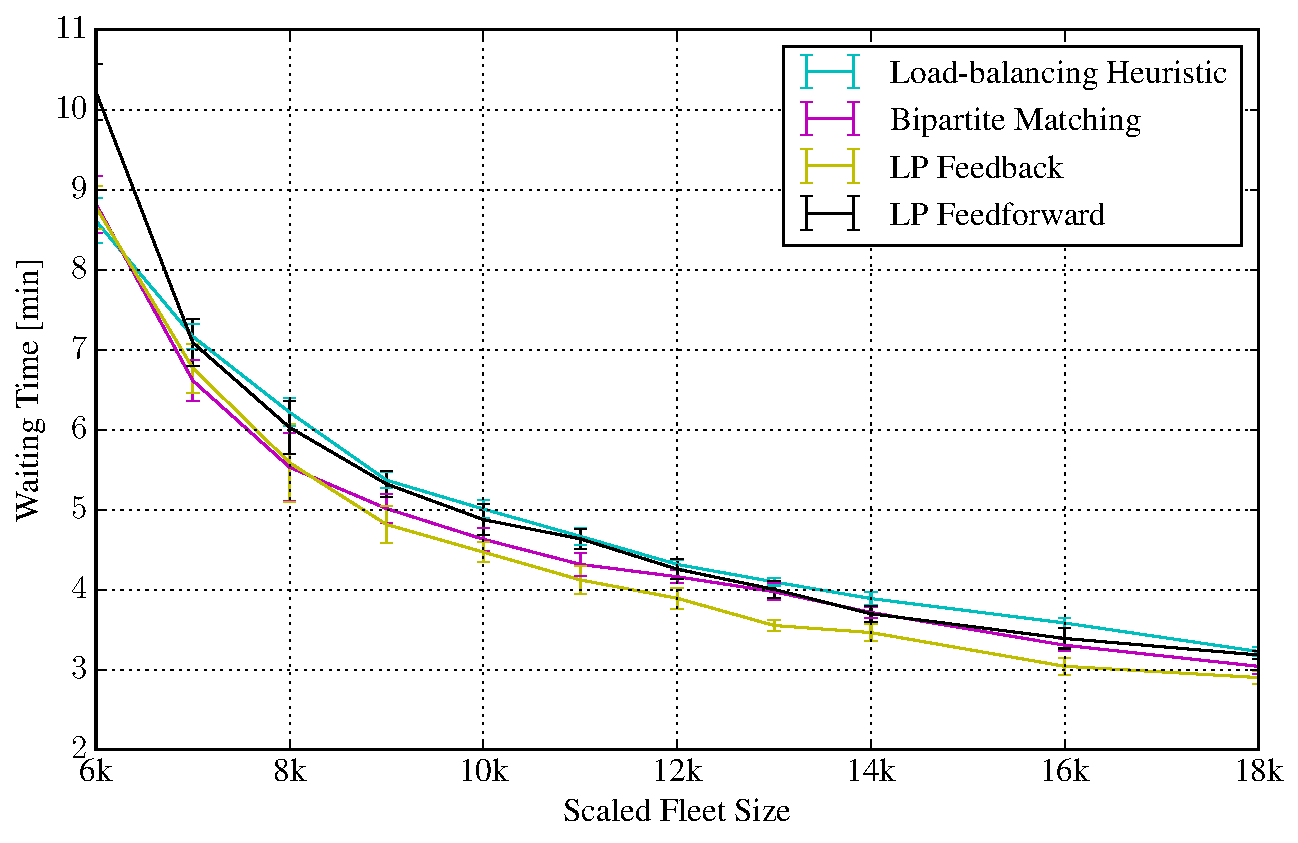
\includegraphics[width=1.0\textwidth]{figures/mean_peak_waiting_times.pdf}
\caption{Average waiting time for an AV to arrive at peak times}
\label{fig:mean_peak_waiting_times}
\end{figure}

Figure \ref{fig:empty_rides} shows the percentage of fleet mileage that is driven without a customer, either for pickup or rebalancing purposes. Clearly, the LP algorithms, which both use rebalancing, have a higher share of empty mileage that the non-rebalancing approaches. The heuristic approach manages to keep the share lowest, since it mainly operates in a best-response state, where only the shortest pickup trips are chosen. Remarkably, the total driven distance for all dispatchers is very similar (Figure \ref{fig:total_distance}), which indicates that the surplus of empty distance for the intelligent dispatchers does not stem from inefficient movements, but rather effective movements towards the expected customer demand for shorter waiting times.

[TODO: Do we need two plots here? Also a plot Total Distance <-> Relative Distance
would be possible, where one can traverse the fleet size along the graph]

\begin{figure}
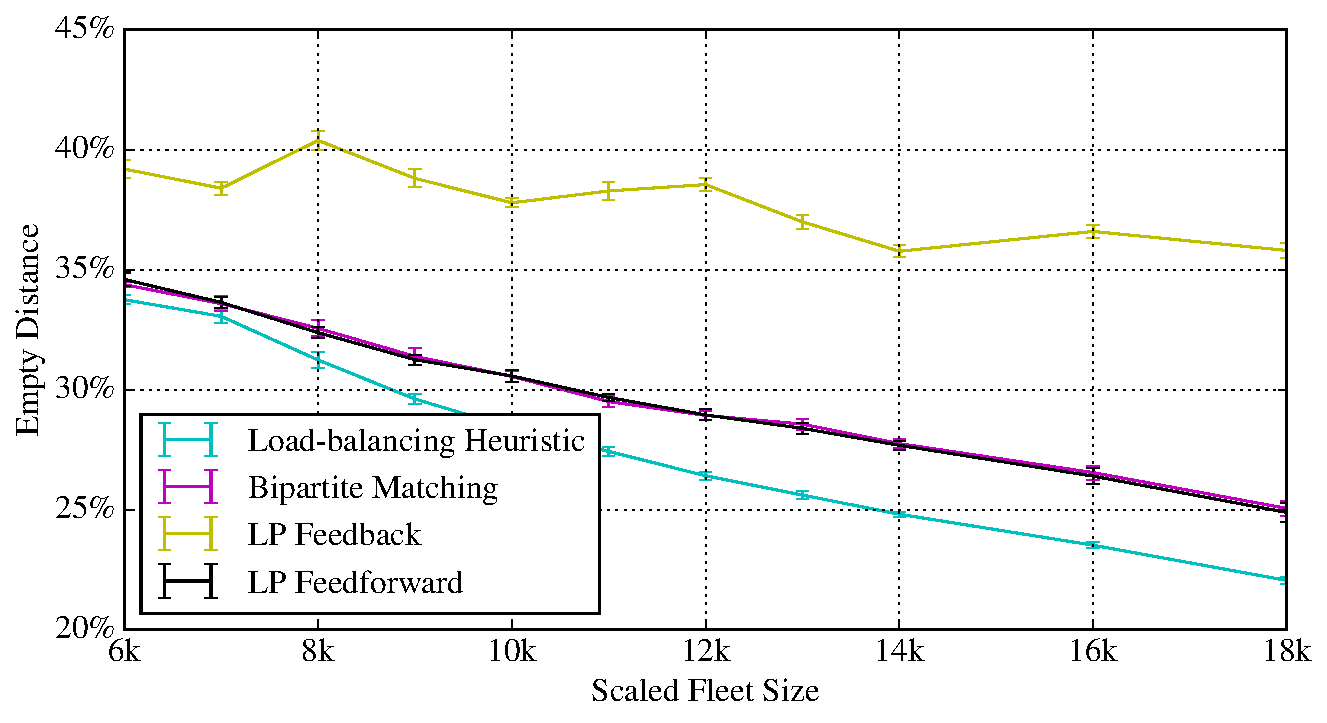
\includegraphics[width=1.0\textwidth]{figures/empty_rides.pdf}
\caption{The fraction of distance that is driven by AVs without a passenger.}
\label{fig:empty_rides}
\end{figure}

\begin{figure}
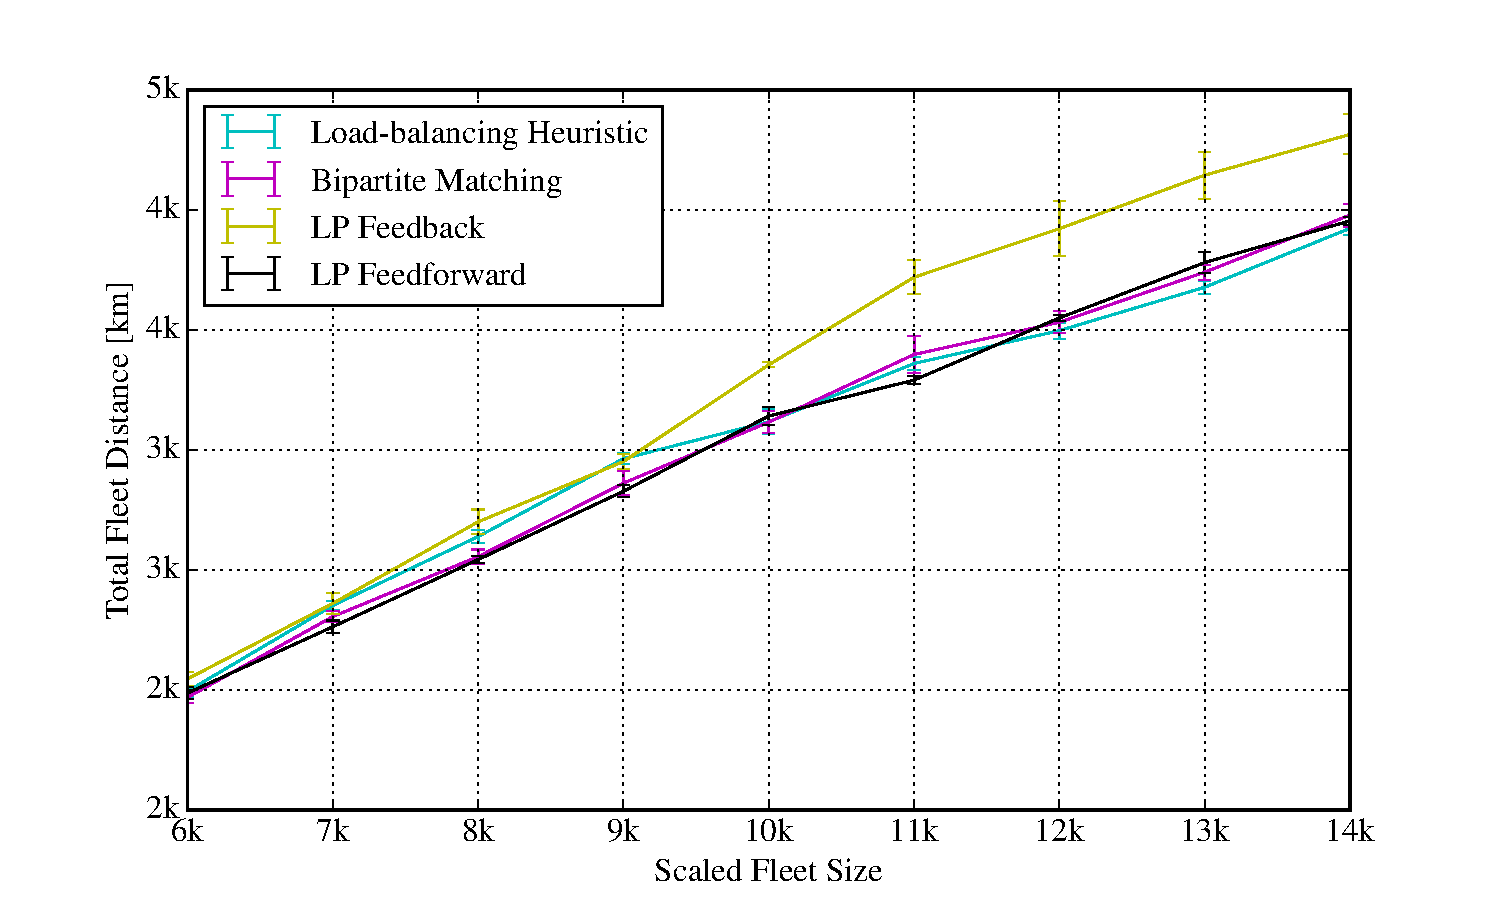
\includegraphics[width=1.0\textwidth]{figures/total_distance.pdf}
\caption{The total distance that is driven by AVs, with and without passenger on-board.}
\label{fig:total_distance}
\end{figure}

Finally, figure \ref{fig:occupancy} shows the occupancy of the fleet for different fleet sizes. Since in the 30h MATSim simulation no AV trips are registered in the hours around midnight, it is possible to correct the resulting 30h occupancy rate to one that is based on a 24h day. As can be seen, the occupancy of all fleet dispatchers exceeds the 8\% that is common today. In general, one can say that the dispatching algorithm has only little influence on fleet occupancy
 [TODO: Trips and Costs are fixed!!]
. The differences lie in the range of 0.5\% between the best and worst performing algorithm, which are the LP Feedback dispatcher and the load-balancing heuristic, respectively. Nevertheless, one can see that the occupancy of the latter is systematically lowest.

\begin{figure}
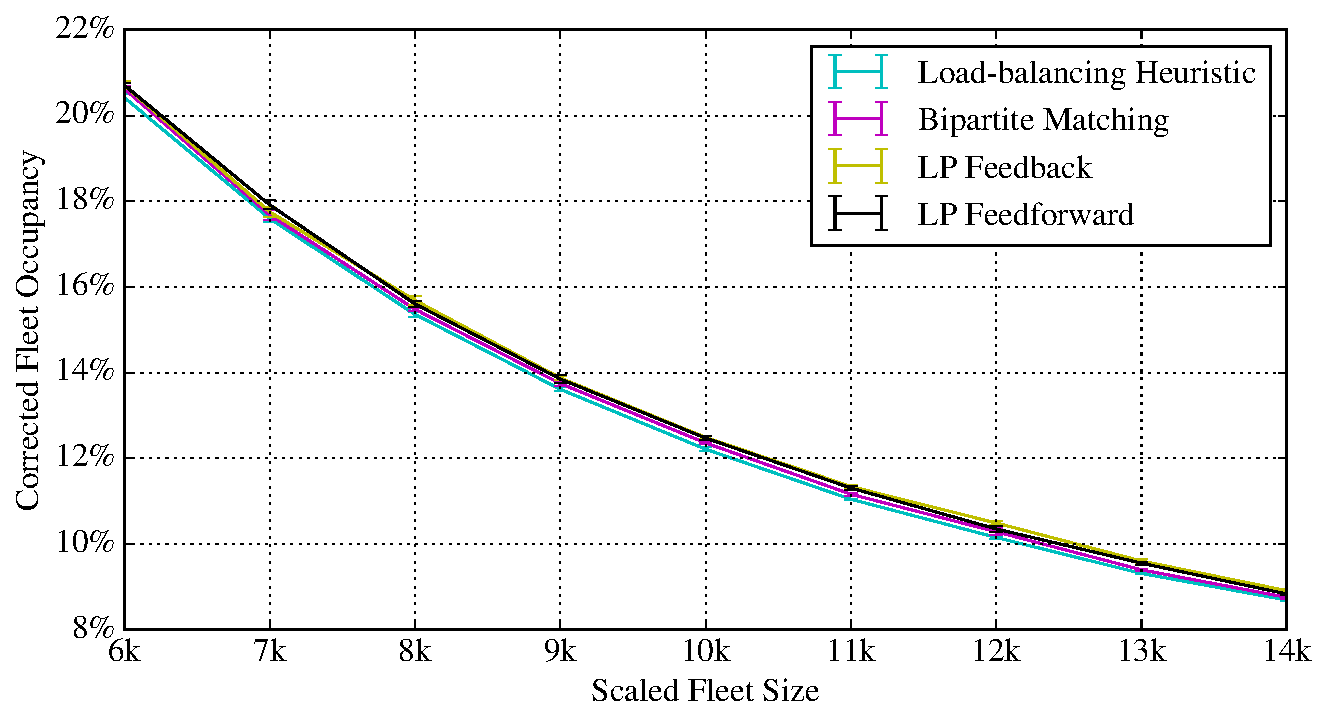
\includegraphics[width=1.0\textwidth]{figures/occupancy.pdf}
\caption{The occupancy of the AV fleet for different flet sizes.}
\label{fig:occupancy}
\end{figure}

\subsection{Cost Analysis}
\label{sec:cost_analysis}

Based on a paper Bösch et al. \cite{cost_paper} the costs of operating the simulated AV services are computed. Specifically, by providing their calculator with key figures of the operator (among them the occupancy, the share of empty rides, the average travel distance) the price that the operator would at least need to ask a customer per kilometer if a profit margin of at least 3\% is targeted. The calculation is based on a detailed analysis of running and fixed costs. Figure~\ref{fig:passenger_price} shows the results from this analysis. Unsurprisingly, the price that needs to be imposed on the customer increases with larger fleet sizes. However, the increase is stronger for the load-balancing heuristic than for any other distpaching strategy. Therefore, with the same fleet being available to an operator, he would be able to offer the service for almost 0.10 CHF less per kilometer than before or save this amount of money.

\begin{figure}
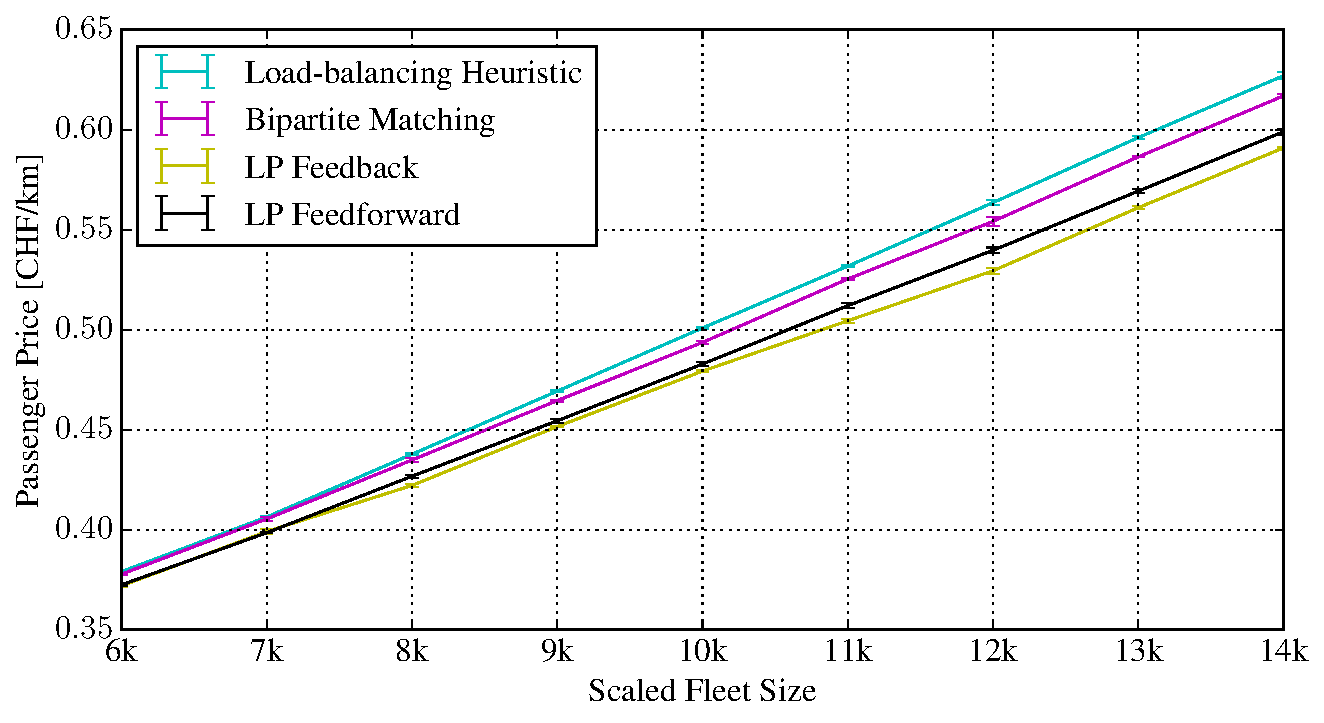
\includegraphics[width=1.0\textwidth]{figures/01_passenger_price.pdf}
\caption{The minimum customer prices that an AV operator needs to charge the customer
in order to have a win margin of at least 3\%.}
\label{fig:passenger_price}
\end{figure}

Compared to the average running costs of driving a private car in Switzerland (around 0.17 CHF/km) 

[todo{variable.. full costs present a nicer story] 

or using public transit (around 0.25 CHF/km) [TODO CITATIONS] the computed prices still seem rather high. Compared to conventional taxi operators, however, the price is extremely low (around 6 CHF/km). Therefore, it is imaginable that the AV service would still be attractive for a large group of people, for which a conventional taxi would be too expensive on a daily basis, but an AV would make such travels affordable.

However, the attractiveness of an AV service does not only depend the price itself, but also on the attitudes of the people towards the service. One key component to the acceptance of an AMoD system is the waiting times that customers need to endure. Figure \ref{fig:time_vs_price} combines the key results from our simulations. There, the price that a specific operator configuration (fleet size and dispatcher) is displayed in comparison to the waiting time that this operator can offer. Assuming that, for instance, a waiting time of five minutes is tolerable, the operator could offer a satisfactory service for around 0.45 CHF with the feedback dispatcher, while he would need to charge 0.50 CHF with the simple load-balancing heuristic. The better the level of service of the operator is ought to be, the larger this margin becomes.

\begin{figure}
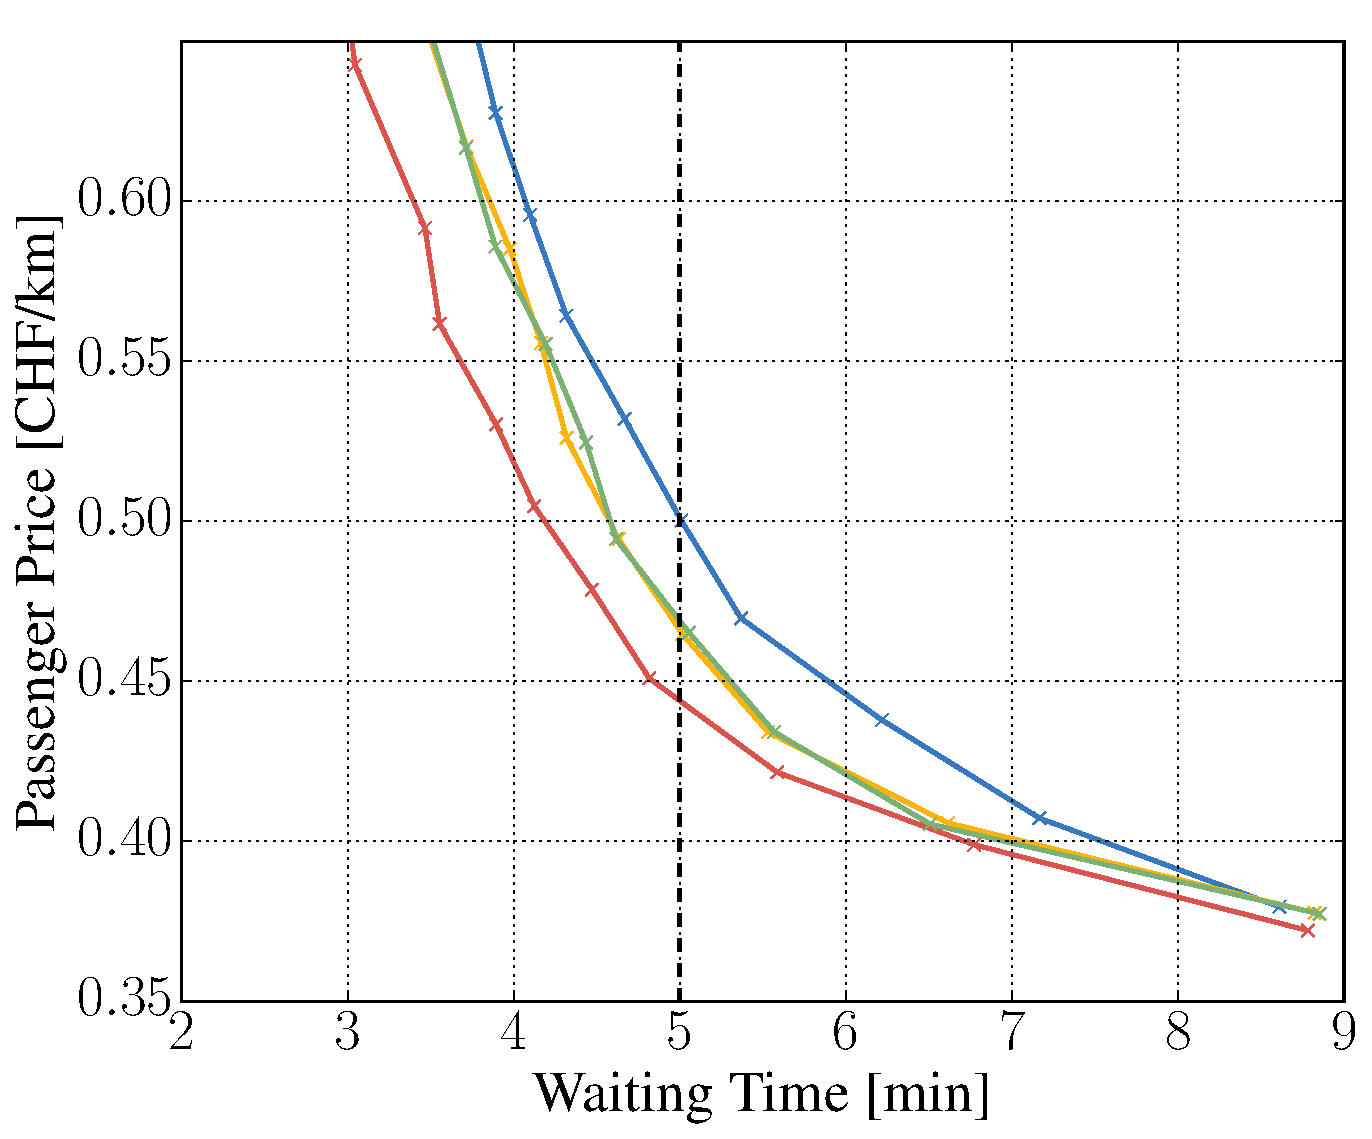
\includegraphics[width=1.0\textwidth]{figures/time_vs_price.pdf}
\caption{Time vs. Price}
\label{fig:time_vs_price}
\end{figure}
